\documentclass[12pt,a4paper]{article}
\usepackage[utf8]{inputenc}
\usepackage[spanish,es-tabla]{babel}
\usepackage{geometry}
\usepackage{graphicx}
\usepackage{multirow}
\usepackage{tabularx}
\usepackage{mathptmx}
\usepackage{fancyhdr}
\usepackage{array}
\usepackage[table]{xcolor}
\usepackage{titlesec}
\usepackage{setspace}
\usepackage{microtype}
\usepackage{lastpage}
\usepackage{booktabs}
\usepackage{enumitem}
\usepackage{amsmath}
\usepackage{amsfonts}
\usepackage{amssymb}

\graphicspath{{images/}{../images/}{./}}

\geometry{
    top=4.7cm,
    bottom=2.5cm,
    left=2.5cm,
    right=2.5cm,
    headheight=3.9cm,
    headsep=0.4cm
}

\setstretch{1.15}
\setlength{\parindent}{0pt}
\setlength{\parskip}{0.45em}
\setlength{\tabcolsep}{4pt}

\titleformat{\section}
  {\normalfont\fontsize{12}{14.5}\bfseries}{\thesection.}{0.6em}{\uppercase}
\titlespacing*{\section}
  {0pt}{1.8ex plus 0.4ex minus 0.2ex}{0.6ex plus 0.2ex}

\titleformat{\subsection}
  {\normalfont\fontsize{11.5}{13.5}\bfseries}{\thesubsection.}{0.5em}{}
\titlespacing*{\subsection}
  {0pt}{1.4ex plus 0.3ex minus 0.1ex}{0.4ex plus 0.1ex}

\titleformat{\subsubsection}
  {\normalfont\fontsize{10.5}{12.5}\bfseries\itshape}{\thesubsubsection.}{0.4em}{}
\titlespacing*{\subsubsection}
  {0pt}{1.1ex plus 0.2ex minus 0.1ex}{0.3ex plus 0.1ex}

\newcolumntype{Y}{>{\centering\arraybackslash}X}
\newcolumntype{L}{>{\raggedright\arraybackslash}X}
\newcolumntype{C}{>{\centering\arraybackslash}X}

\definecolor{headerred}{RGB}{180, 0, 0}
\definecolor{darkred}{RGB}{140, 0, 0}
\definecolor{lightgraybg}{RGB}{248, 248, 248}
\definecolor{tableheader}{RGB}{232, 238, 246}

\newcommand{\docCodigo}{TI-SIGE-ENT-S2-007}
\newcommand{\docVersion}{1.0}
\newcommand{\docProceso}{CIERRE DE FASE / CONSOLIDACIÓN SEMANA 2}
\newcommand{\docElaboracion}{04/09/2026}
\newcommand{\docRevision}{PENDIENTE DE REVISIÓN}
\newcommand{\docTitulo}{ENTREGABLE GENERAL Y CONSOLIDADO DE LA SEMANA 2}
\newcommand{\docOrganizacion}{FACULTAD DE INGENIERÍA EN SISTEMAS, ELECTRÓNICA E INDUSTRIAL}
\newcommand{\docSubOrganizacion}{CARRERA DE INGENIERÍA DE SOFTWARE}

\newcommand{\encabezadofrecuente}{%
    \renewcommand{\arraystretch}{1.15}%
    \noindent\makebox[\textwidth][c]{%
    \begin{tabularx}{\textwidth}{|>{\centering\arraybackslash}m{2.8cm}|Y|>{\centering\arraybackslash}m{4.8cm}|}
        \hline
        \multirow{4}{2.8cm}{\centering\raisebox{-1.15cm}{
\includegraphics[width=2.5cm,height=2.0cm,keepaspectratio]{images/logo.png}}}
        & \textbf{\fontsize{9}{11}\selectfont \docOrganizacion} 
        & \textbf{\fontsize{8}{10}\selectfont CÓDIGO:} \fontsize{8}{10}\selectfont \docCodigo \\
        \cline{3-3}
        & \textbf{\fontsize{8.5}{10.5}\selectfont \docSubOrganizacion} 
        & \textbf{\fontsize{8}{10}\selectfont VERSIÓN:} \fontsize{8}{10}\selectfont \docVersion \\
        \cline{2-3}
        & \textbf{\fontsize{8}{10}\selectfont PROCESO:} \fontsize{8}{10}\selectfont \docProceso 
        & \textbf{\fontsize{8}{10}\selectfont ELABORACIÓN:} \fontsize{8}{10}\selectfont \docElaboracion \\
        \cline{2-3}
        & \textbf{\fontsize{8.5}{10.5}\selectfont \docTitulo} 
        & \textbf{\fontsize{8}{10}\selectfont ÚLTIMA REVISIÓN:} \fontsize{8}{10}\selectfont \textbf{\textcolor{darkred}{\docRevision}} \\
        \hline
    \end{tabularx}%
    }%
}

\pagestyle{fancy}
\fancyhf{}
\fancyhead[C]{\encabezadofrecuente}
\fancyfoot[C]{\fontsize{10}{12}\selectfont Página \thepage\ de \pageref{LastPage}}
\renewcommand{\headrulewidth}{0pt}

\begin{document}

\section{Título}
\textbf{Denominación del Entregable:} Informe Consolidado de Cierre de Fase de Diseño, Arquitectura y Modelado Técnico (EDT 2.7)

\vspace{0.15cm}
\noindent
\textbf{Ficha Técnica de Identificación:}
\begin{itemize}[leftmargin=1.5em, itemsep=1.5pt, topsep=1.5pt]
    \item \textbf{Código Documental:} \docCodigo \quad | \quad \textbf{Versión:} \docVersion
    \item \textbf{Institución:} Universidad Técnica de Ambato (UTA) -- FISEI
    \item \textbf{Carrera:} Ingeniería de Software (Séptimo Semestre "A")
    \item \textbf{Módulo Académico:} Gestión de Proyectos de Software
    \item \textbf{Docente Tutor:} Ing. Paulo Torres
    \item \textbf{Fecha de Elaboración:} \docElaboracion \quad | \quad \textbf{Estado:} \textbf{\textcolor{darkred}{Aprobado}}
    \item \textbf{Período de Ejecución:} Semana 2 (25/08/2026 al 04/09/2026)
    \item \textbf{Equipo de Trabajo:} Steeven Toala (Líder / Arquitecto), Heidy Villavicencio (Analista / UI-UX), Nixon Hurtado (Backend / DBA), Andrea Vasquez (Frontend / QA)
\end{itemize}

\section{Introducción}
Durante la \textbf{Semana 2: Diseño Rápido y Arquitectura}, el equipo de desarrollo completó con éxito el 100\% de los modelos de diseño técnico, estructural y visual del sistema \textbf{SIGE}. Se definieron los diagramas UML de Casos de Uso, la Clean Architecture en .NET 9, los diagramas de interacción de secuencia/actividades/clases con el modelado formal de FirmaEC, el modelo relacional normalizado en PostgreSQL 16, el sistema de diseño visual en Figma y la orquestación completa de servicios en Docker Compose.

\section{Objetivo}

\subsection{Objetivo General}
Consolidar formalmente los artefactos de diseño técnico, arquitectónico y de interfaz de usuario generados en la Semana 2, certificando la viabilidad técnica y el cumplimiento de la línea base arquitectónica para habilitar el inicio de la Fase 3 de Construcción y Desarrollo Core.

\subsection{Objetivos Específicos}
\begin{itemize}[leftmargin=1.5em, itemsep=1.5pt]
    \item Verificar la finalización y aprobación técnica de los 6 paquetes de trabajo EDT de la Semana 2.
    \item Establecer la trazabilidad entre los casos de uso, la Clean Architecture en .NET 9 y el esquema de persistencia en PostgreSQL 16.
    \item Consolidar la distribución del esfuerzo invertido por el equipo (72 horas de ingeniería).
\end{itemize}

\section{Alcance}

\subsection{Límites del Consolidado (In-Scope)}
\begin{itemize}[leftmargin=1.5em, itemsep=1.5pt]
    \item Abarca la totalidad de artefactos de diseño y arquitectura producidos entre el 25 de agosto y el 04 de septiembre de 2026 (EDT 2.1 al EDT 2.6).
\end{itemize}

\subsection{Exclusiones (Out-of-Scope)}
\begin{itemize}[leftmargin=1.5em, itemsep=1.5pt]
    \item No incluye el código fuente de controladores o endpoints definitivos ni migraciones aplicadas en base de datos (competencia de la Semana 3).
\end{itemize}

\section{Definiciones}
\begin{itemize}[leftmargin=1.5em, itemsep=2pt]
    \item \textbf{Clean Architecture:} Patrón arquitectónico que promueve la separación de responsabilidades en capas concéntricas con la regla de dependencia hacia el dominio.
    \item \textbf{EDT (\textit{Estructura de Desglose del Trabajo}):} Descomposición jerárquica del proyecto orientada a entregables verificables.
    \item \textbf{Docker Compose:} Herramienta para definir y ejecutar aplicaciones Docker multicontenedor en entornos de desarrollo local y pruebas.
\end{itemize}

\section{Responsabilidades}
\begin{itemize}[leftmargin=1.5em, itemsep=2pt]
    \item \textbf{Steeven Toala (Líder / Arquitecto):} Consolidación del informe general, revisión de Clean Architecture y cierre de fase.
    \item \textbf{Heidy Villavicencio (Analista / UI-UX):} Validación de casos de uso, especificación UX y diagramas de interacción.
    \item \textbf{Nixon Hurtado (Backend / DBA):} Verificación del modelo de datos ER, scripts DDL y orquestación Docker.
    \item \textbf{Andrea Vasquez (Frontend / QA):} Revisión de prototipos visuales Figma y criterios de accesibilidad WCAG 2.1 AA.
    \item \textbf{Ing. Paulo Torres (Docente Tutor):} Supervisión técnica y aprobación de la línea base de diseño y arquitectura.
\end{itemize}

\section{Normativa Legal y Técnica}
\begin{itemize}[leftmargin=1.5em, itemsep=2pt]
    \item \textbf{ISO/IEC/IEEE 42010:2011:} Descripción de arquitectura de sistemas y software.
    \item \textbf{ISO/IEC 25010:} Requisitos de calidad y evaluación del software.
    \item \textbf{Guía del PMBOK (7ma Edición):} Gestión del Alcance e Integración de Proyectos.
\end{itemize}

\section{Método, Políticas y Contenidos}
El flujo de dependencia de los artefactos producidos durante la Semana 2 se resume en la arquitectura consolidada de entregables:

\begin{figure}[htbp]
    \centering
    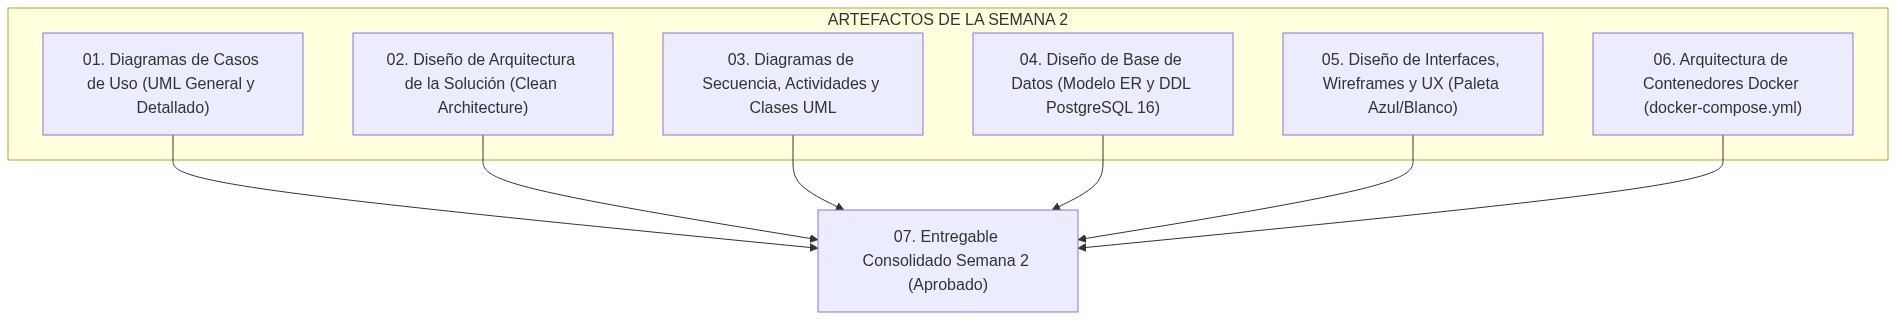
\includegraphics[width=0.85\textwidth,height=4.8cm,keepaspectratio]{images/s2_07_consolidado_s2.png}
    \caption{Mapa de Entregables Consolidados y Línea Base de la Semana 2.}
    \label{fig:s2_07_cons}
\end{figure}

\section{Descripción de actividades}

\subsection{Índice de Entregables de la Semana 2 (Estructura EDT)}
\begin{enumerate}[leftmargin=1.5em, itemsep=2.5pt]
    \item \textbf{EDT 2.1 -- Diagramas de Casos de Uso (UML General y Detallado):} Modelado UML de interacciones por roles institucionales y especificación formal de casos de uso críticos (CU-03A/B/C en cascada, CU-04 y CU-18).
    \item \textbf{EDT 2.2 -- Diseño de Arquitectura de la Solución (Clean Architecture):} Especificación de Clean Architecture en .NET 9, separación de capas (\texttt{Domain}, \texttt{Application}, \texttt{Infrastructure}, \texttt{WebAPI}), patrones de diseño y JWT.
    \item \textbf{EDT 2.3 -- Diagramas de Secuencia, Actividades y Clases UML:} Modelado dinámico de Validation Gates, API de Firma Electrónica con FirmaEC en cascada de 3 escalones, ciclo de vida del Plan al Informe y clases de dominio.
    \item \textbf{EDT 2.4 -- Diseño de Base de Datos (Modelo ER y DDL PostgreSQL 16):} Diagrama Entidad-Relación (ERD) en 3FN para PostgreSQL 16, diccionario de datos de 9 entidades e índices DDL de rendimiento.
    \item \textbf{EDT 2.5 -- Diseño de Interfaces, Wireframes y UX (Paleta Azul/Blanco):} Sistema de diseño Azul y Blanco institucional, wireframes de las 3 vistas por rol y accesibilidad WCAG 2.1 AA.
    \item \textbf{EDT 2.6 -- Arquitectura de Contenedores Docker (docker-compose.yml):} Archivo \texttt{docker-compose.yml} completo con PostgreSQL, MinIO S3, LanguageTool y scripts de inicio.
\end{enumerate}

\subsection{Distribución de Trabajo y Cumplimiento del Equipo}

\begin{table}[htbp]
\centering
\small
\begin{tabularx}{\textwidth}{|>{\hsize=0.7\hsize\bfseries}X|>{\hsize=1.0\hsize}X|>{\hsize=0.45\hsize\centering\arraybackslash}X|>{\hsize=1.2\hsize}X|>{\hsize=0.65\hsize\centering\arraybackslash}X|}
    \hline
    \rowcolor{tableheader}
    Integrante & Rol Principal & Horas & Tareas Culminadas & Estado \\
    \hline
    Steeven Toala & Líder de Proyecto / Arquitecto & 20 h & Clean Architecture, C4, Docker Compose, Clases UML & \textbf{100\% Completo} \\
    \hline
    Heidy Villavicencio & Analista de Requerimientos / UI-UX & 18 h & Casos de Uso, Wireframes Figma, Secuencias & \textbf{100\% Completo} \\
    \hline
    Nixon Hurtado & Desarrollador Backend / DBA & 18 h & Modelo ER PostgreSQL, Diccionario Datos, MinIO Init & \textbf{100\% Completo} \\
    \hline
    Andrea Vasquez & Desarrolladora Frontend / QA Tester & 16 h & Diseño de Componentes React, Accesibilidad UX & \textbf{100\% Completo} \\
    \hline
    \rowcolor{gray!15}
    \textbf{TOTAL SEMANA 2} & \textbf{Equipo de Desarrollo SIGE} & \textbf{72 h} & \textbf{6 Paquetes de Trabajo EDT} & \textbf{Aprobado} \\
    \hline
\end{tabularx}
\caption{Matriz de Control de Esfuerzo y Desempeño - Semana 2.}
\label{tab:s2_07_esfuerzo}
\end{table}

\subsection{Conclusión y Transición a la Semana 3 (Desarrollo Core)}
Con la culminación de la Semana 2, el proyecto \textbf{SIGE} queda formalmente preparado para el inicio del desarrollo e implementación transaccional, arrancando en la \textbf{Semana 3} con las migraciones de Entity Framework Core, los seeders del catálogo institucional SGC, los servicios de autenticación JWT/RBAC y el cliente React 19 con Vite.

\vspace{0.3cm}

% =============================================================
% FIRMAS DE RESPONSABILIDAD
% =============================================================
\section{Firmas de Responsabilidad}

\noindent
\renewcommand{\arraystretch}{1.2}
\begin{tabularx}{\textwidth}{|>{\raggedright\arraybackslash}m{2.9cm}|>{\raggedright\arraybackslash}X|>{\centering\arraybackslash}m{4.6cm}|>{\centering\arraybackslash}m{2.3cm}|}
    \hline
    \rowcolor{headerred}
    \textcolor{white}{\textbf{ACCIÓN}} & \textcolor{white}{\textbf{NOMBRE Y CARGO}} & \textcolor{white}{\textbf{FIRMA}} & \textcolor{white}{\textbf{FECHA}} \\
    \hline
    \textbf{Elaborado por:} & Steeven Toala\newline \textit{Líder de Proyecto / Arquitecto Software} & \parbox[c]{4.4cm}{\centering\vspace{4pt}
\includegraphics[height=1.5cm,width=4.0cm,keepaspectratio]{images/firma_steveen.png}\vspace{4pt}} & 04/09/2026 \\
    \hline
    \textbf{Revisado por:} & Steeven Toala\newline \textit{Líder de Proyecto / Arquitecto Software} & \parbox[c]{4.4cm}{\centering\vspace{10pt}\textbf{\textcolor{gray!80}{\scriptsize [ PENDIENTE DE REVISIÓN ]}}\vspace{10pt}} & \textbf{\textcolor{gray!90}{Pendiente}} \\
    \hline
    \textbf{Aprobado por:} & Ing. Paulo Torres\newline \textit{Docente Tutor - Gestión Proyectos Software} & \parbox[c]{4.4cm}{\centering\vspace{10pt}\textbf{\textcolor{gray!80}{\scriptsize [ PENDIENTE DE APROBACIÓN ]}}\vspace{10pt}} & \textbf{\textcolor{gray!90}{Pendiente}} \\
    \hline
\end{tabularx}

\vspace{0.4cm}

% =============================================================
% CONTROL DE CAMBIOS
% =============================================================
\section{Control de Cambios}

\noindent
\renewcommand{\arraystretch}{1.2}
\begin{tabularx}{\textwidth}{|>{\hsize=0.45\hsize\centering\arraybackslash}X|>{\hsize=1.55\hsize\raggedright\arraybackslash}X|>{\hsize=1.2\hsize\raggedright\arraybackslash}X|>{\hsize=0.8\hsize\centering\arraybackslash}X|}
    \hline
    \rowcolor{gray!20}
    \textbf{Versión} & \textbf{Descripción del cambio} & \textbf{Responsable del cambio} & \textbf{Fecha de aprobación} \\
    \hline
    1.0 & Consolidación final de entregables de la Semana 2 / Pendiente de revisión & Steeven Toala & \textbf{\textcolor{gray!90}{Pendiente de Revisión}} \\
    \hline
\end{tabularx}

\vspace{0.4cm}

\section{Anexos}
\subsection*{Anexo 1: Acta de Cumplimiento del Hito de Diseño y Arquitectura}
Se certifica la entrega formal de los 6 documentos técnicos de la Semana 2 para revisión por el docente tutor de la cátedra de Gestión de Proyectos de Software.

\end{document}
